\documentclass[letterpaper]{article}
\title{The Infamous Particle Filter\\16-831 HW3: Fall 2011}
\author{Natasha Kholgade, Heather Knight, and Marynel V\'azquez}
\date{}
\usepackage[margin=1in]{geometry}
\usepackage{amsmath}
\usepackage{amssymb}
\usepackage{url}
\usepackage{graphicx}
\usepackage{color}
\usepackage{subfigure}
% Make URL click-able
\usepackage{hyperref}

% Draft for now
%\usepackage{draftwatermark}
%\SetWatermarkLightness{ 0.95 }
%\SetWatermarkScale{ 5 }

% Don't indent after paragraphs
\parindent 0in

\begin{document}

\maketitle

\section{Introduction}

In this assignment, we address the problem of localizing a lost robot
within a known map, given its odometry and laser rangefinder data. We
implement a particle filter that (1) initializes N particles, (2) uses
odometry measurements as principal input to the robot's motion model,
(3) uses laser ray casting to assess particle quality with respect to
real world laser measurements, (4) resamples
the particles when the weight variance
rises about a threshold. Particle filters are great for situations in
which we have sensor and motion data from a known map but no ground
truth. We observe good localization performance with a choice of $800-1000$
particles and noise parameters of $\alpha_1=.03, \alpha_2=.03,
\alpha_3=.01, \alpha_4=.01$ for the motion model. As our
videos demonstrate, our implementation worked successfully on the first and 
second data logs.
% NOTE: We did not test in all provided data sets.. only log 1 and 2...
%% Particle filters are great for situations in
%% which we have sensor and motion data from a known map but no ground
%% truth. We observe good localization performance with a choice of $800$
%% particles and noise parameters of $\alpha_1=.03, \alpha_2=.03,
%% \alpha_3=.01, \alpha_4=.01$ for the motion model. As the accompanying
%% videos demonstrate, our implementation worked successfully on all of
%% the provided data sets.

\section{Implementation}

We implement almost our entire system in MATLAB, except for the ray
casting algorithm. We implement the latter in C++, since it is
computationally intensive. We use MATLAB Executable (MEX files) to
bridge the gap between the two programming environments.

\subsection{Particle Initialization}

Given that the dataset depicts a robot traveling through a building,
we can assume that the robot was always inside either a room or the
hallway.  Thus, we generate our initial samples as a uniform
distribution over all pixels that are known but unoccupied with a
probability of one (see Fig. \ref{fig1}).  
% NOTE: When did this happen? Where are we assigning zero weights?
%% In the next section we use
%% similar reasoning to infer the benefits of discarding (i.e. assign a
%% zero weight to) any particles that go outside the building during the
%% motion modeling.

\begin{figure}[h!tbp]
\centering
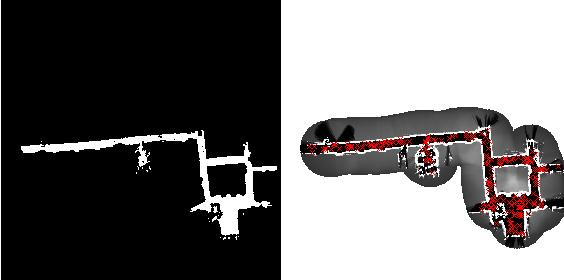
\includegraphics[width=0.8\linewidth]{gen_particles}
\caption[.]{Particle Initialization: (left) map of all pixels that are known but unoccupied 
with a probability of one, (right) full map with initialization with 200 particles}
\label{fig1}
\end{figure}

\subsection{Motion Model}

We use the motion model described in Thrun et al. [1] in this
assignment. Our motion model uses the odometry data only to estimate
the motion relative to the current particle frames. also incorporating
Gaussian noise to model the presence of inaccuracies in the odometry
sensing. Figure \ref{fig2} depicts results from our motion model testing phase.

\begin{figure}[h!tbp]
\centering
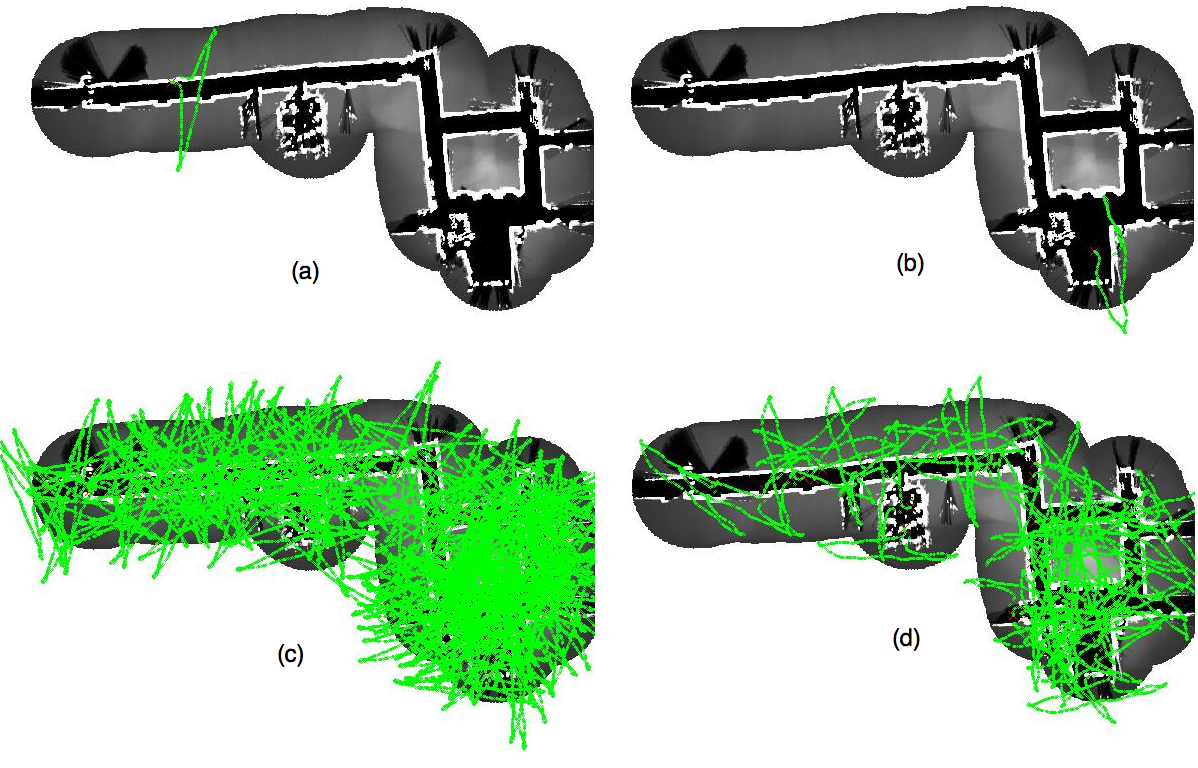
\includegraphics[width=0.8\linewidth]{all_motionmodel}
\caption[.]{Motion Model for (a) one particle with no noise, 
(b) one particle with noise, (c) 200 particles no noise, (d) 200 particles with noise
}
\label{fig2}
\end{figure}
\subsubsection{The Motion Equations}

To get motion estimates from one odometry configuration
$(\tilde{x},\tilde{y},\tilde{\theta})$ to another
$(\tilde{x}',\tilde{y}',\tilde{\theta}')$ on a two dimensional plane,
the robot needs to perform a rotation to align with the direction of
travel, a translation along that direction, and a rotation to adjust
itself to the final orientation (Figure \ref{fig3}).

\begin{figure}[h!tbp]
\centering
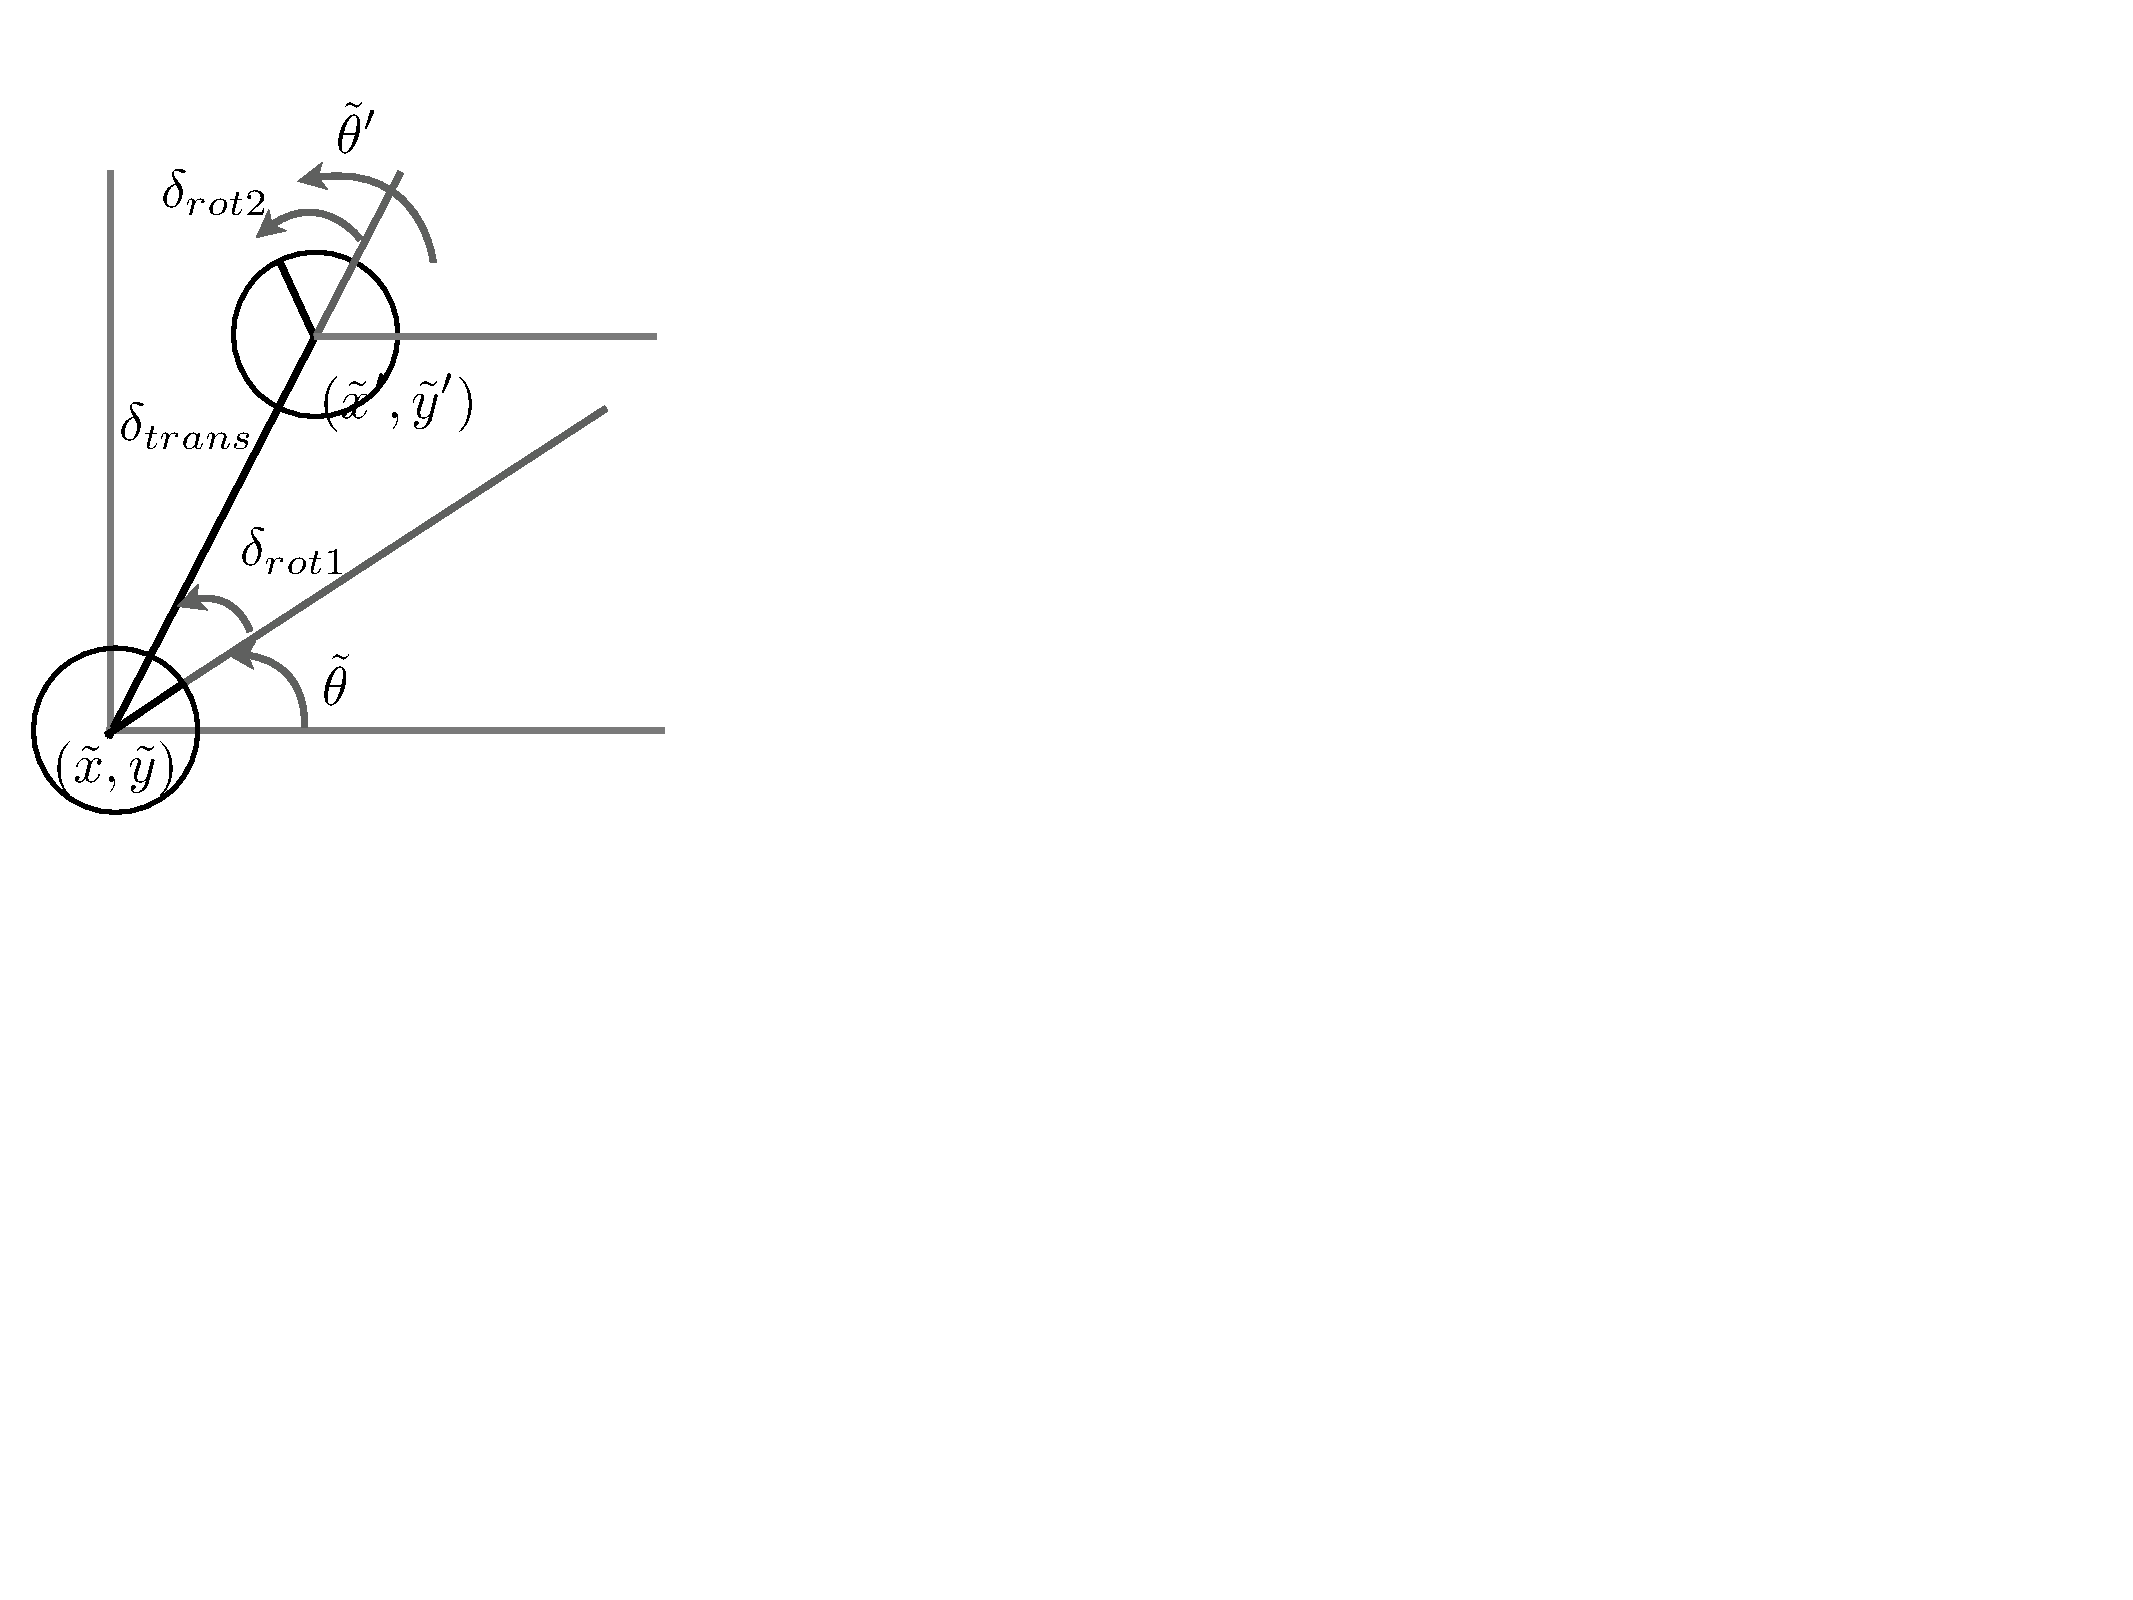
\includegraphics[width=.3\linewidth]{motionmodel}
\caption[.]{Motion model for a robot moving from configuration
  $(\tilde{x},\tilde{y},\tilde{\theta})$ to
  $(\tilde{x}',\tilde{y}',\tilde{\theta}')$}
\label{fig3}
\end{figure}

The initial change in rotation can be specified as:
$$\delta_{rot1}=\text{atan2}(\tilde{y}'-\tilde{y},\tilde{x}'-\tilde{x})-\tilde{\theta}$$
The change in translation is the distance travelled between the initial and final locations:
$$\delta_{trans}=\sqrt{(\tilde{x}'-\tilde{x})^2+(\tilde{y}'-\tilde{y})^2}$$
The final change in rotation is given as
$$\delta_{rot2}=\tilde{\theta}'-\tilde{\theta}-\delta_{rot1}$$

\subsubsection{Incorporating Noise}
We assume that the actual values of rotation and translation can be
described by removing independent noise $\epsilon_b$ with zero mean
and variance $b$:
$$ \hat{\delta}_{rot1}=\delta_{rot1}-\epsilon_{\alpha_1 \left|\delta_{rot1}\right|+\alpha_2 \left|\delta_{trans}\right|}$$
$$ \hat{\delta}_{trans}=\delta_{trans}-\epsilon_{\alpha_3 \left|\delta_{trans}\right|+\alpha_4 \left|\delta_{rot1}+\delta_{rot2}\right|}$$
$$ \hat{\delta}_{rot2}=\delta_{rot2}-\epsilon_{\alpha_1 \left|\delta_{rot2}\right|+\alpha_2 \left|\delta_{trans}\right|}$$
The updates to the translation and rotation are given by:
$$x'=x+\hat{\delta}_{trans}\cos(\theta+\hat{\delta}_{rot1})$$
$$y'=y+\hat{\delta}_{trans}\sin(\theta+\hat{\delta}_{rot1})$$
$$\theta'=\theta+\hat{\delta}_{rot1}+\hat{\delta}_{rot2}$$

\subsubsection{Sampling Distribution}

We obtain all our samples from a normal distribution centered around the quantity of interest:

$$x \sim \mathcal{N}(\overline{x}, \sqrt{b})$$

To obtain a random sample according to the normal distribution, we randomly generate a set of $12$ values from the uniform distribution between -1 and 1, sum them, and multiply by the factor $b/6$ where $b$ is the variance of the distribution.

\subsubsection{Training the $\alpha's$}

We found that having larger noise for the rotation parameters $\alpha_1$ and $\alpha_2$ versus the translation parameters $\alpha_3$ and $\alpha_4$ was important.  The rotation space for all possible $\alpha's$ given the number of particles we have is very large, thus we found small rotation parameters made it unlikely that our particles would happen to be at the best orientations. Small horizontal and vertical translation errors were easier to recover from by comparison.

\subsubsection{Validation}

We tested the motion model individually before integration. As shown
in Figure \ref{fig2}, first we generated a single particle and ran the
the motion model without noise. Its motion mimicked the motion from
the odometry data as expected. Next, we added noise to the motion
model, and increased the number of particles. When the particles were
initialized at the same position and the motion model ran with noise,
we obtained a satisfactory banana-shaped spread.

% NOTE: I am very confused about the particles being resilent :( maybe
%it's my non-native English that's making this hard on me?
%% Contrasting the many
%% particles with noise case in Fig. 2 to that without, you see how an
%% enough particles can be resilient against inaccuracies in the odometry
%% data because there are variations in the particle actions. One sees
%% this even better by initializing a bunch of particles to the same
%% starting point and observing the spread. When a satisfactory
%% banana-shaped spread was obtained, we moved on to the next step.

\subsection{Sensor Model}

We implemented three different methods for assessing the sensor
model. First, we focused on a simple probabilistic map model. Consider
a particle with laser position $[x\ y\ \theta]$, and a laser
measurement $L = [l_0\ \ldots\ l_{179}]$. We computed where the laser beams fall
 in the map as follows:
\begin{equation*}
\big( \forall_{i}\ |\ i \in \mathbb{N}^0 \wedge 0 \leq i < 180 \ |
\alpha = i\pi/180 \ \wedge\ map\_pos_i = [x + l_i\cos(\alpha),\ y + l_i\sin(\alpha)]\big)
\end{equation*}
and then we extracted the occupancy probabilities for all these
places:
\begin{equation*}
o_i = smoothed\_map(round(map\_pos_i*scale))\mbox{, with } scale = 1/10
\end{equation*}
Note that a smoothed version of the occupancy map ($smoothed\_map$)
was used instead of the original values. This typically helps beams
that fall close to an occupied space in the map, but not exactly.\\

The weight of the particle was finally obtained in this approach by summing and
exponentiating the probabilites $o_i$ for all beams. \\

Particles tended to move outside of the free space in the map with our
first implementation. We considered a reduced number of uniformly
distributed beams from the full measurement to make the independence
assumption more reasonable, but our results did not
improve. To try to accommodate this situation, we decided to use the
number of hits for a laser measurement, instead of the occupancy
probabilities directly. This meant transforming $o_i$ to either
$0$ or $1$, depending on whether beam $i$ falls in a free or occupied
space in the map:
\begin{equation*}
hit_i = 
\begin{cases}
1 \mbox{, if } o_i >= H\\
0 \mbox{, if } o_i < H
\end{cases}
\end{equation*}
typically with $H = 0.9$. We then summed up and exponentiated the
number of hits to compute the weight of the
particle.\footnote{Exponentiation was useful to avoid zero weights.}\\

After several tests, we could not get our second approach to work.
Particles did not remain in the unoccupied space of the map, even
after ignoring laser beams with values outside the expected
range. The maximum expected value for a laser measurement was
  always set to $8000$ cm, while the minimum varied from $0$ to
  $50$.\\

After limited success, we elected to implement a ray tracing based
method, first in MATLAB and then in C++. 

% NOTE: I think the following paragraph can be simplified  by just
% mentioning the expected range value for the laser measurements. If
% you feel something is missing from above, then uncomment...
%% To ensure the overall solution would consistently converge, there
%% were also several pre-processing steps that were important to
%% implement carefully.  The original sampling of the environment by
%% the sensor data was highly non-uniform. In particular, there were a
%% large number of points in close proximity to the robot and fewer
%% points far from the robot.  If the likelihood was calculated over
%% all of these data points, the information carried by points farther
%% away would be overshadowed by the large quantity of near points. In
%% addition, the laser itself has a max range, and so there are
%% frequent artificial peaks at 8000cm. To remedy these problems, we
%% filtered the points along the path of the ray.

%% NOTE: We never implemented this version...  \subsubsection{Simple
%% Probabalistic Map Model} When an observation is made, the laser
%% data is projected into the smoothed map from each particle
%% location.  In our first model, the sensor model assumes
%% independence between all laser points so the likelihood of a scan
%% is taken to be the product of the likelihoods of each of the
%% individual points. (Note that the laser on the robot is
%% approximately 25 cm offset forward from the true center of the
%% robot.) The likelihood of each ray containing a successful hit is
%% computed as a mixture of a normal and a uniform
%% distribution: $$Lpoint = z_{hit} * prob(dist, \sigma_{hit}) +
%% z_{uniform} $$ The above $z�s$ are the weights used in mixing the
%% distributions and $prob(dist, \sigma_{hit})$ computes the
%% probability of the distance to the nearest obstacle under a
%% zero-mean Gaussian distribution with standard deviation
%% $\sigma_{hit}$. The $z_{uniform}$ term allows for the rejection of
%% noise at the cost of slowing down convergence. \\ Note that we
%% smooth the map beforehand to improve results but this smoothing is
%% not performed at each time step, as that would increase computation
%% significantly. Instead the map can be smoothed once for all
%% particles at the beginning of the particle filter.

\subsubsection{Ray tracing Model}

The weight for a particle is computed from the difference between the
laser measurement $L$ (captured in the real world by the robot) and an \textit{ideal} measurement $\hat{L}$
taken from the position of the particle in the map. The process goes
as follows: (1) we ray cast laser beams from the laser position
$[x\ y\ \theta]$ of a particle, then (2) we find the location where the
rays hit for the first time an obstacle in the map, and (3) finally
use the distances from the the laser position to the hit locations as
the components of the ideal laser measurement.\\

We process all laser beams $i$, with $i=1 \ldots 179$, as detailed below:
\begin{align*}
& beamAngle_i = \theta + i*\pi/180 - \pi/2 \hspace{3em}\mbox{// beams start from
    right to left}\\
& orientation_i = [cos(beamAngle_i), sin(beamAngle_i)]\\
& curr\_step = step\\
& \mbox{while } curr\_step < maxL :\\
& \hspace{3em} beamEnd_i = laser\_position + orientation_i *
  currStep\\
& \hspace{3em} o_i = map(floor(beamEnd_i*scale))\\
& \hspace{3em} \mbox{if } \mbox{isUnknown}(o_i): \\
& \hspace{6em} beamEnd = laser\_position + orientation*maxL\\
& \hspace{6em} break\\
& \hspace{3em} \mbox{elif } o_i > H: \\
& \hspace{6em} break \\
& \hspace{3em} \mbox{endif}\\
& \hspace{3em} curr\_step += curr\_step \\
& \mbox{end}\\
& distance_i = norm_2(laser\_position - beamEnd_i)
\end{align*}

The variables $scale$, $step$, $maxL$, and $H$ represent the map
scale, the  step to move
forward along the beam,\footnote{The step is chosen small enough so
  that no cell in the occupancy map is skipped along the ray.} the maximum allowed range value and the
occupied probability threshold, respectively. The function
$\mbox{isUnknown}(.)$ tells wheter the occupancy probability $o_i$ is
outside the allowed $[0,1]$ range.\footnote{Some occupancy values in
  the map are unknown.}\\

The values $distance_i$ compose the ideal laser measurement $\hat{L} =
[distance_0\ \ldots \ distance_{179}]$. Typically, $\hat{L}$ would
have 180 components, but if some values in the real laser measurement
$L$ are outside the expected range, then their respective beams are
ignored both for $L$ and $\hat{L}$.\\

To obtain a value for the weight of a particle we first subtract $L$
and $\hat{L}$. This operation gives us the differences in range per
beam. Then we compute probabilities for the differences under a Normal
distribution with zero-mean and variance $\sigma_{beam}$. Ideally, all
differences would be zero, hence the zero mean, but to overcome
measurement noise we allow some variation in the readings using
$\sigma_{beam}$. Finally, we sum all probabilities and exponentiate.  In
other words,
\begin{equation*}
w = exp(\sum_i(\mathcal{N}(L_i - \hat{L_i}; 0, \sigma_{beam})))
\end{equation*}

% Explained this with more details above.. the subsampling is
% mentioned in the validation subsection
%%  ray casting beams and comparing the distances to occupied spaces
%% along the rays in the map with laser measurements. The probability
%% for a hit is computed using a normal distribution centered at the
%% laser measurement for a beam (with $\sigma = \sigma_{beam}$).
%% First we filter the beams that do not meet the minimum and max
%% thresholds. Next, we cast the ray linearly out from the particle
%% location, ensuring that the hit characteristics occur at the first
%% object or wall encountered rather than giving a false positive for
%% an obstructed feature that its lasers would not be able to
%% sense. Given this data over all possible particle rays (literally
%% 180 beams, although we subsample by a factor of four).
%% \subsubsection{Computing Weights}
%% Weights using the probabilities from the map-based sensor model: $W = sum(hitProb)$ \\
%% Weights counting thresholded probabilities from map: $W = sum(hitProb > 0.8)+epsilon$ \\
%% Weights from ray casting: $W = exp(sum(probs,2))$ 

\subsubsection{Validation}

We created an interactive point and click interface to validate the
ray casting model. Using the application, we positioned different
particles on the map, and run our ray casting algorithm for each of
them. Images such as the right-most in Figure \ref{fig4} were obtained
during this testing phase.\\

\begin{figure}[h!tbp]
\centering
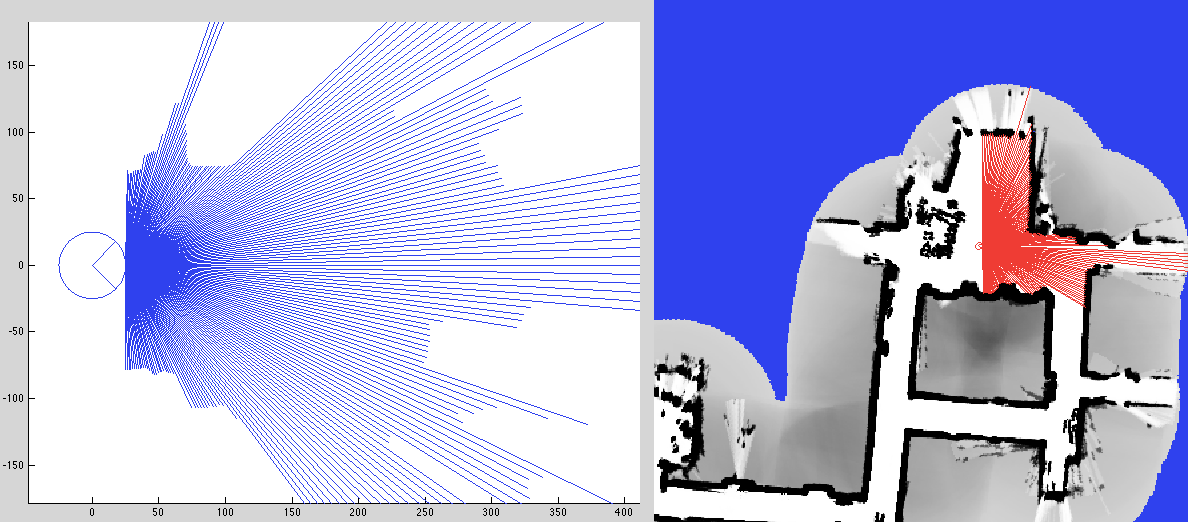
\includegraphics[width=.9\linewidth]{laser}
\caption[.]{Laser data visualization: (left) real laser measurement,
  (right) ray casting result }
\label{fig4}
\end{figure}

% NOTE: Elaborated above..
%% It took many steps to integrate our sensor model into the overall
%% particle filter, but before that we isolated the functioning of the
%% Sensor Model itself by creating a point and click interface to insert
%% oriented particles into the map and estimate the rays from that
%% center.  Other steps we used to validate its functioning included A, B
%% and C. [FEEL FREE TO ELABORATE]\\

We assume laser beams are independent, and designed our code to allow
for measurement subsampling. We ran tests of the sensor model using
all 180 beams, but also using every other beam (90 in total) and
less. We corroborated later that skipping too many beams (e.g., more than
4) in favor of more independence between measurements did not improve
our results. \\

Once we were confident in the sensor model itself, integrating this
step into the overall particle filtering functioning involved many
iterations of parameter testing. Challenges we faced were choosing how
often to resample (discussed in the next section), evaluating $\alpha$
values to fit the sensor model, and matching up coordinate systems
across the code of the various project contributors.

\subsection{Resampling Step}

As discussed in class, we used Normalized Importance Resampling to
redistribute the particles over the previous particle space in a
manner that reflects their overall probability levels as expressed by
the particles� most recent weights.  

\subsubsection{Methodology}

Specifically, for the $N$ particles we create $N$ bin indices by using
their normalized weights to create a continuous PDF. We accomplish
that by creating a cumulative sum of weights for each sequential
particle. Next, we generate a random number between zero and one as
the first resampling position, using the continuous PDF index of that
location to assign the first particle in our new set of
particles. After that we iterate $N-1$ times, moving our sampling
position forward by $1/N$ with a circular buffer. When resampling is
complete, we match our new particles with the stored indices and reset
all weights.

\subsubsection{Resampling Frequency}
We do not resample the particles at explicit timestep, but rather
track the overall variance in the weights and only perform resampling
when this number has surpassed a certain threshold. We
experimentally determine a good variance threshold by tracking how
long it took unlikely particles or particle clusters to die out, while
maintaining enough diversity in the particle distribution to allow
reliable convergence. \\

 Resampling too often can lead to lack of particle diversity and thus loss of information, not resampling enough means the algorithm will not converge and means fewer additional particles will be added to the true particle location, which could make that true particle location less robust to noise.

\section{Algorithm Summary}

Our particle filter code consists of the following steps:

% NOTE: I took out the smoothing. We don't smooth with the raycast
% sensor model. Move the resampling to the end. Removed the move
% forward particle on Laser data (we never implemented that). There
% were a lot of steps in that algorithm that we didn't implement.
\begin{verbatim}
 Generate N particles using a uniform distribution over the unoccupied \
   positions in the map and all possible headings.  
 
 While there is still data:
   If next reading is Odometry data:
      Sample particles using the motion model.
      Move any particle that goes off the map to the border.
   If next reading is Laser data:
      Filter the laser data (e.g, ignore beams outside of expected range)
      Compute weight for each particle using the ray casting approach 
   If weights variance is above threshold:
      Resample particles (and set new particle weights to 1/N)
\end{verbatim} 
It also generates the map and sensor
 visualization for each step along the way.

\section{Results}

\begin{figure}[ht]
\centering
\subfigure[]{
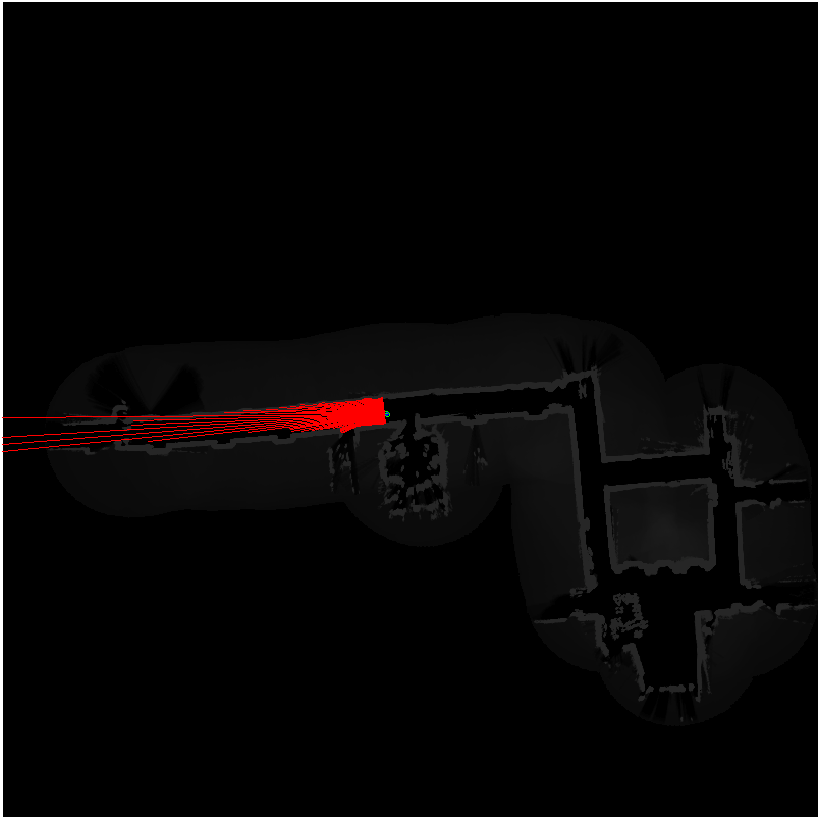
\includegraphics[scale=.15]{start.png}
\label{fig:subfig1}
}
\subfigure[]{
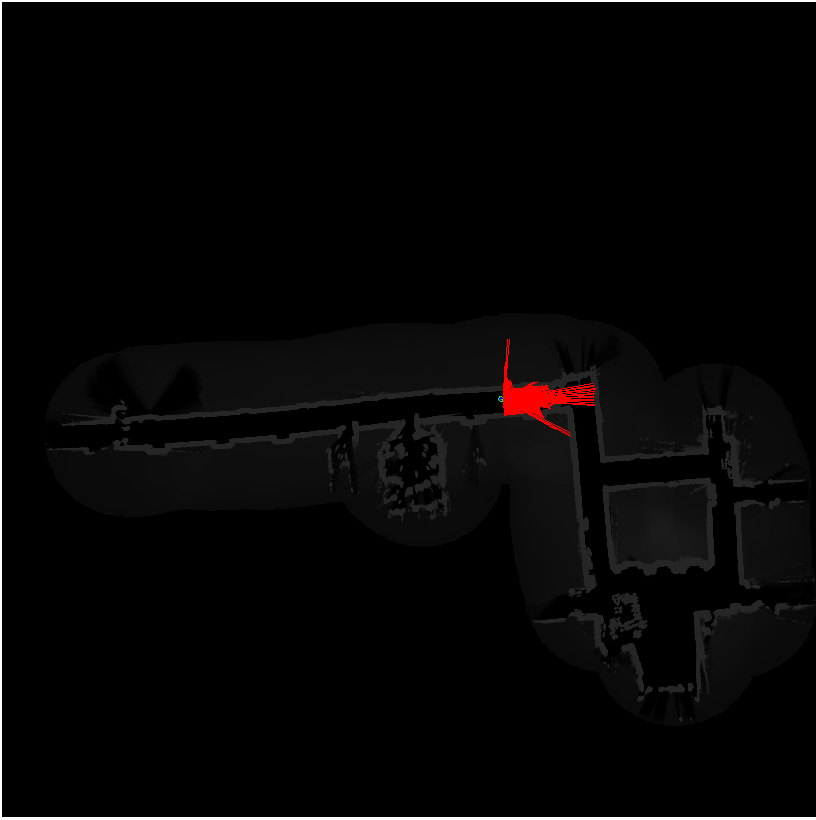
\includegraphics[scale=.15]{mid.png}
\label{fig:subfig2}
}
\subfigure[]{
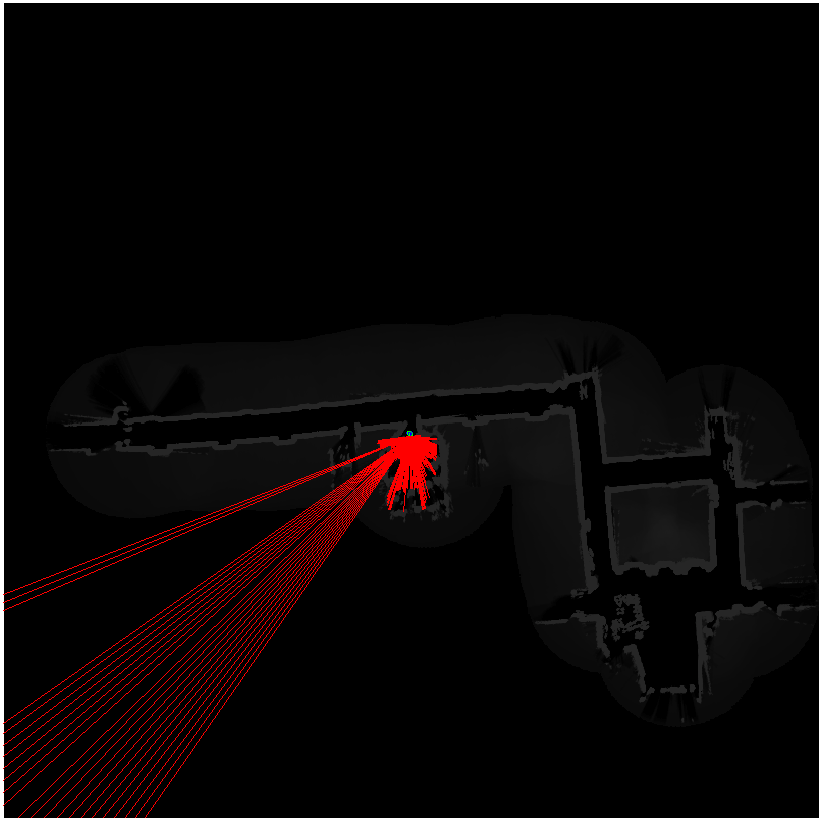
\includegraphics[scale=.15]{end.png}
\label{fig:subfig3}
}
\label{fig:subfigureExample}
\caption[Optional caption for list of figures]{Plots of the robot's location for `robotdata2.log' at frames \subref{fig:subfig1} 270 (few frames into the start of the route), \subref{fig:subfig2} 3670 (midway), and \subref{fig:subfig3} 5360 (final frame)}
\end{figure}
 
As the accompanying videos demonstrate, our implementation worked successfully on the logs `robotdata1.log' and `robotdata2.log'.  Note: to execute our accompanying code, use the script: 
\begin{verbatim}runParticleFilter\end{verbatim}

Before using the code, execute at the command prompt
\begin{verbatim}./compile.sh\end{verbatim}

which is located in the same directory (change the include path in the 'compile.sh' script to point to your version of MATLAB), and then call
\begin{verbatim}mex CXX=g++ -lm particle.o vector2D.o raycast.cpp -output raycast\end{verbatim}

before running the particle filter.\\

As the movies show, our particle filter algorithm converges to the correct global position within around $200$ iterations. We depict the particles as blue dots. For the highest likelihood particle,  we plot an oriented circle with triangle depicting laser location and use its pose to transform the filtered laser data into red beams in the world coordinates. For the first data log, we used $1000$ particles, and for the second data log, we used $800$ particles. We found that noise parameters $\alpha_1=.03, \alpha_2=.03, \alpha_3=.02, \alpha_4=.02$, and a resampling threshold of $2.5 - 3.5 \times 10^{-5}$ for the standard deviation of the weights worked best to produce the desired results.

\section*{References}

[1] Thrun, S., Burgard, W., and Fox, D. \emph{Probabilistic Robotics}, The MIT Press, 2005. 

\end{document}
